%%%%%%%%%%%%%%%%%%%%%%%%%%%%%%%%%%%%%%%%%%%%%%%%%%%%%%%%%%%%%%%%%%%%%%%%%%%%%%%
% Author:  Pablo Alvarado
%
% Escuela de Ingeniería Electrónica
% Instituto Tecnológico de Costa Rica
%
% Tesis de Licenciatura
% 
% Phone:   +506 550 2106
% Fax:     +506 591 6629
% email:   palvarado@ietec.org
%
% $Id: main.tex 1513 2010-08-15 01:25:24Z palvarado $
%
%Versión modificada por Yeiner Arias para uso en
%la Escuela de Ingeniería Mecatrónica
%%%%%%%%%%%%%%%%%%%%%%%%%%%%%%%%%%%%%%%%%%%%%%%%%%%%%%%%%%%%%%%%%%%%%%%%%%%%%%%

\documentclass[12pt,twoside,letterpaper]{book}

\usepackage[utf8]{inputenc}
\usepackage{ifthen}                     % provide if-then-else operators

% --------------------------------------------------------------------------
% Global variables required in document formatting
% --------------------------------------------------------------------------

\newboolean{bookmode}                  
\setboolean{bookmode}{true}

\newboolean{draftmode}                  
\setboolean{draftmode}{false}

% GENERAL AUTHOR, TITLE AND KEYWORDS
\newcommand{\scriptAuthor}{Diego Brenes Poveda}
\newcommand{\scriptTitle}{Diseño de un sistema multi-USV autónomo para muestreo y monitorización ambiental en entornos acuáticos} 
\newcommand{\scriptKeywords}{palabras, clave, ...}

\newcommand{\boxeditorial}{%
}

\newcommand{\pdfAuthor}{\scriptAuthor}
\newcommand{\pdfTitle}{\scriptTitle} 
\newcommand{\pdfKeywords}{\scriptKeywords}

% --------------------------------------------------------------------------

% include all packages and define all required general macros
\input{macros}
\allowdisplaybreaks[3]

% --------------------------------------------------------------------------
\begin{document}
  \graphicspath{{./}{./fig/}}

  \pagenumbering{alph}
  \renewcommand{\tablename}{Tabla}
  \renewcommand{\listtablename}{\'Indice de tablas}
  \renewcommand{\examplesolution}{Solución}
  \pagestyle{empty}

  \include{titlepage}
  \include{disclaimer}
  \include{resumen}
  \include{dedicatoria}
  \chapter*{Agradecimientos}
\thispagestyle{empty}

En esta sección van los agradecimientos a personas dirigidas(redactar).
\vspace*{1cm}

\scriptAuthor

Cartago, \today

\cleardoublepage

%%% Local Variables: 
%%% mode: latex
%%% TeX-master: "paMain"
%%% End: 


  %----------------------------------------------------------------------------
  \frontmatter
  %----------------------------------------------------------------------------
  \pagestyle{fancy}

  \pdfbookmark[1]{Indice General}{Indice General}
  \parskip0ex

  \tableofcontents
  \cleardoublepage

  \phantomsection
  \addcontentsline{toc}{chapter}{Lista de figuras}
  \listoffigures
  \cleardoublepage

  \phantomsection
  \addcontentsline{toc}{chapter}{Lista de tablas}
  \listoftables
  \cleardoublepage

\ifdraft{%
  \listoftodo
}{%
}

  \include{notation}    % símbolos o fórmulas matemáticas
  \include{glosario}    % opcional; renombrar para evitar conflicto con abreviaciones

  \parskip1.3ex

  %----------------------------------------------------------------------------
  \mainmatter
  %----------------------------------------------------------------------------

  \graphicspath{{./}{./fig/}}

  %% ---------------------------------------------------------------------------
%% intro.tex
%%
%% Introduction
%%
%% $Id: intro.tex 1477 2010-07-28 21:34:43Z palvarado $
%% ---------------------------------------------------------------------------

\chapter{Introducción}
\label{chp:intro}

\section{Contexto}

El presente proyecto se enmarca en el proyecto HAERA (Hybrid AERial Aquatic robotic system for sampling, monitoring and intervention) de la Universidad de Sevilla, 
que busca avanzar hacia un sistema robótico híbrido aéreo-acuático para muestreo, monitorización e intervención ambiental\cite{Cite2}. Se desarrolla de forma presencial en la 
Escuela Técnica Superior de Ingeniería (ETSI) de dicha universidad \cite{Cite1}, bajo la asesoría de profesores-tutores del Departamento de Ingeniería de Sistemas y Automática, 
en colaboración con el grupo de investigación Multi-Robot and Control Systems (MACS)\cite{Cite3}, especializado en cooperación multi-robot, planificación y control de robots, 
y control no lineal, robusto y adaptativo, con experiencia previa en proyectos multi-robot internacionales y nacionales orientados a aplicaciones medioambientales 
y de inspección.

Para su ejecución, la ETSI dispone de las instalaciones de laboratorio del grupo MACS, que proveen el equipamiento y los recursos necesarios para la integración y 
validación de los sistemas desarrollados, entre ellos las plataformas USV (Unmanned Surface Vehicles) base sobre las que se construye la solución \cite{Cite3}. Las pruebas de 
campo se realizan en cuerpos de agua cercanos a la ciudad de Sevilla, entorno natural para la validación del sistema bajo condiciones reales de operación.

\newpage

\section{Descripción del Problema}

La contaminación de ríos, lagos y océanos, originada por asentamientos humanos, actividades agrícolas e industriales, continúa degradando los ecosistemas acuáticos 
sin que existan, en la mayoría de los casos, herramientas fiables para su monitorización en tiempo real. Esta carencia adquiere especial relevancia considerando que 
más de un tercio de la población mundial carece de acceso a saneamiento mejorado, lo que refuerza la necesidad de datos ambientales de calidad para respaldar la 
gestión de recursos hídricos y la detección temprana de contaminantes\cite{Cite5}.

La ausencia de mecanismos de monitorización sostenida y en tiempo real tiene consecuencias directas sobre la salud de los ecosistemas acuáticos: sin un monitoreo 
adecuado a escala, el daño ambiental resultante puede volverse permanente e irreversible, mientras los cuerpos de agua continúan actuando como sumidero y conducto de 
contaminación antropogénica sin que se generen los datos necesarios para intervenir a tiempo \cite{Cite6}. Esta limitación retrasa la identificación temprana de contaminantes 
y reduce la capacidad de los organismos responsables para tomar decisiones de gestión basadas en información actualizada.

Los sistemas robóticos disponibles actualmente para atender esta necesidad presentan limitaciones documentadas. Los drones aéreos, si bien permiten cubrir grandes 
áreas, alcanzan tasas de éxito de muestreo de entre el 60 {\%} y el 83 {\%} debido a su incapacidad de interactuar directamente con el agua \cite{Cite4}. Por su parte, los vehículos 
aéreo-acuáticos híbridos existentes presentan un tamaño considerable, un costo elevado y una maniobrabilidad reducida, lo que restringe su aplicabilidad en cuerpos de 
agua de difícil acceso. Estas limitaciones evidencian un vacío en la literatura respecto a plataformas multi-robot validadas en condiciones acuáticas no controladas\cite{Cite2}.

\section{Síntesis del Problema}

En el marco del proyecto HAERA, se dispone de plataformas USV base desarrolladas en el laboratorio. Sin embargo, estas carecen de los subsistemas necesarios para operar 
como una flota autónoma orientada a la monitorización y el muestreo de datos en entornos acuáticos reales, limitación documentada como un vacío en plataformas multi-robot 
validadas en condiciones no controladas \cite{Cite2}. Del análisis de las causas asociadas a esta limitación se priorizaron tres causas críticas: la falta de algoritmos de navegación 
autónoma por "waypoints" integrados en la flota, la ausencia de sensores de percepción específicos para misiones de monitorización ambiental acuática, y la falta de 
integración de las plataformas USV base con hardware embarcado modular. Estas tres causas constituyen el eje sobre el cual se estructuran los objetivos del presente proyecto.

El desarrollo del proyecto se enmarca en un periodo de ejecución limitado, condicionado a la adaptación de las plataformas USV ya disponibles en el laboratorio, a la 
variabilidad ambiental de los cuerpos de agua cercanos a Sevilla y al cumplimiento de la normativa española aplicable. Como supuesto crítico, se asume que dichas plataformas 
son adaptables a la integración requerida y que la infraestructura del laboratorio del grupo MACS estará disponible durante toda la ejecución.

Resolver esta limitación permitirá ampliar la cobertura espacial, aumentar la redundancia operativa y mejorar la fiabilidad del muestreo en cuerpos de agua reales. Los 
datasets recolectados en condiciones reales constituirán además un recurso de alto valor para el grupo MACS y para grupos de investigación afines, sentando las bases para 
que organismos de gestión ambiental e instituciones públicas dispongan a futuro de herramientas más confiables para la monitorización autónoma de cuerpos de agua.



\section{Objetivos y estructura del documento}

\index{objetivos}

\subsection{Objetivo General}

Diseñar un sistema multi-USV autónomo que permita ejecutar misiones cooperativas de recolección de datos ambientales en entornos acuáticos.

\subsection{Objetivos Específicos}

\begin{itemize}
    \item Analizar el estado actual de las plataformas USV del laboratorio del grupo MACS para definir los requerimientos oficiales del sistema multi-USV.
    \item Diseñar la arquitectura de integración del hardware embarcado y de los sensores de percepción en al menos dos USVs para habilitar la operación autónoma 
          estable de la plataforma y la adquisición continua de datos ambientales en condiciones controladas de laboratorio.
    \item Implementar la arquitectura de comunicaciones y navegación autónoma cooperativa de la flota multi-USV para habilitar la coordinación simultánea de al menos dos vehículos.
    \item Evaluar el desempeño cooperativo de la flota multi-USV mediante pruebas de integración en un entorno de simulación y en el laboratorio del grupo MACS.
\end{itemize}

\newpage

\subsection{Estructura del documento}

A continuación, se presenta un esquema de las secciones que conforman este documento, junto con una breve descripción de su contenido.

\begin{itemize}
    \item Capítulo 1: Se introduce el contexto del proyecto, definiendo el problema a resolver y los objetivos planteados.
    \item Capítulo 2: Se presenta el marco teórico, con los conceptos fundamentales relevantes para el diseño e implementación del sistema multi-USV.
    \item Capítulo 3: Se expone la metodología de diseño empleada, justificando los procedimientos seguidos para la selección de las alternativas técnicas del sistema.
    \item Capítulo 4: Se detalla la propuesta de diseño, documentando la arquitectura del sistema multi-USV y la integración de sus subsistemas.
    \item Capítulo 5: Se presentan y analizan los resultados obtenidos en las pruebas de validación en simulación y en laboratorio, junto con el análisis económico del proyecto.
    \item Capítulo 6: Se presentan las conclusiones y recomendaciones derivadas del desarrollo del proyecto.

\end{itemize}

El principal aporte de ingeniería de este proyecto radica en la integración y validación de una arquitectura multi-USV autónoma y cooperativa, donde se combinan 
hardware embarcado, sensores de percepción, comunicaciones inalámbricas y navegación por "waypoints" sobre plataformas acuáticas reales, contribuyendo a cerrar el 
vacío identificado en la literatura respecto a sistemas multi-robot validados en condiciones acuáticas no controladas.
  \chapter{Marco Teórico}
\label{ch:marco}

\section{Descripción}

Toda tesis hace referencia a trabajos previos en el área y trabajos afines que
están directamente relacionados con lo planteado en la tesis.

Además, en el marco teórico debe aparecer la información absolutamente
necesaria para comprender la solución, y por eso es recomendable escribir
primero la solución (el siguiente capítulo), para ir anotando qué debe ser
explicado en el marco teórico.

\subsection{Redacción}

La \nt{redacción} en todo el documento debe seguir un estilo científico
objetivo. Esto implica que se redacta de modo impersonal, sin utilizar primeras
personas del singular o del plural, y se evita el uso de cualquier tipo de
calificativo, sustituyéndolos siempre por datos concretos, vinculados a
referencias bibliográficas o datos experimentales. Los comparativos también
deben concretarse a hechos y datos, y nunca dejarse ``en el aire''. Por la
naturaleza de la tesis, el tiempo verbal es usualmente presente, no perdiendo
nunca de vista que se está explicando ``cómo hacer algo'', en vez de ``qué se
hizo''.

Las \nt{frases} deben ser cortas, y debe evitarse que el lector tenga que saltar
constantemente entre partes de la tesis, lo que implica una exposición lineal
clara, donde lo que se necesita ya ha sido explicado antes. Deben evitarse
redundancias y por tanto cada concepto se exponen en un único lugar.

Todo aspecto circunstancial es irrelevante para la tesis, es decir, si se ha
desarrollado en el laboratorio $X$, o en el curso $Y$, con el profesor $Z$, o
en la empresa $W$, el nombre de funciones o clases en su código, etc., es
información irrelevante para reproducir el experimento, y por lo tanto sobra.
Numeración del documento

La primera página de la tesis es la correspondiente a la introducción, así que
ésta debe ser la página 1. Desde la introducción, hasta antes de la
bibliografía, las unidades son ``Capítulos''. La bibliografía y anexos no se
consideran capítulos, así que ya no continúan con la misma numeración de los
capítulos (la paginación sí continua). Los índices, notación, glosario, etc. se
numeran con números romanos en minúscula (i,ii,iii,iv,v,vi...) y antes del
índice (portada, resúmenes, agradecimientos, hoja de evaluadores, etc.) las
páginas no llevan numeración. 

Esta plantilla LaTeX ya se ocupa de todo lo anterior.

\subsection{Ecuaciones}

Para citar \nt{ecuaciones} se utilizan paréntesis redondos, y no es necesario emplear la palabra ``ecuación''. Por ejemplo ``Introduciendo en (4.2) los resultados de (3.3) y (3.7) se obtiene ...''. La ecuación es parte del flujo de texto y no un objeto flotante, así que no pueden emplearse como figuras. Cuando se requiere la ecuación, allí se inserta \eqref{eq:QP}.

\begin{equation}\label{eq:QP}
    \begin{split}
     \min_{\boldsymbol{x}_{k+1}, \boldsymbol{u}_{k}} \quad \boldsymbol{J}&= \left (\boldsymbol{x}_{k+1} - \boldsymbol{x}^{*}\right )^{T}{\boldsymbol{Q}}\left (\boldsymbol{x}_{k+1} - \boldsymbol{x}^{*}\right )\\&+\left ( \boldsymbol{u}_{k}- \boldsymbol{u}^{*} \right )^{T}\boldsymbol{R}\left ( \boldsymbol{u}_{k}- \boldsymbol{u}^{*} \right ) \\  \mathrm{s.a.} \quad \boldsymbol{x}_{k+1}&={\boldsymbol{A}}\boldsymbol{x}_{k} + {\boldsymbol{B}}_{k} \boldsymbol{u}_{k} + {\boldsymbol{d}}_{k} \\
     \boldsymbol{G}\boldsymbol{u}_{k} &\geq \boldsymbol{W}
    \end{split}
\end{equation}

También puede utilizar el editor de ecuaciones en línea.

\subsection{Figuras}

Para el almacenamiento de imágenes existen dos tipos de formato: las imágenes
raster y las imágenes vectoriales.\index{imagen!raster}

Las imágenes raster son representadas por una rejilla de píxeles, en donde cada
píxel tiene un valor que representa al nivel de gris o el color. La
discretización espacial es ineludible, y la única forma de obtener buena
calidad es empleando tamaños grandes de la imagen que conduzcan a resoluciones
de al menos 300 puntos por pulgada en la impresión, lo que conlleva a archivos
de documentos de varios megabytes. Dentro de los formatos para almacenar
imágenes raster existen algunos con pérdida (como el JPEG) que producen en
imágenes sintéticas, como diagramas, estructuras ruidosas que dan una
apariencia de baja calidad a las figuras. Otros formatos (como PNG, BMP, TIFF o
GIF) no tiene pérdidas de información, pero los algoritmos de compresión no
pueden reducir el tamaño de las imágenes con los mismos factores de reducción
que los formatos con pérdidas. Este tipo de formatos debe utilizarse únicamente
para fotografías o capturas de escenas reales con cámaras digitales.

\index{imagen!vectorial}
Las imágenes vectoriales \textbf{deben} ser empleadas en todo tipo de
diagrama. En ellas no se almacenan píxeles, sino las estructuras geométricas
que componen la figura como círculos (representado por posicion de su centro y
su radio), rectángulos (representados por sus esquinas), líneas, texto, etc. La
mayoría de programas para elaborar este tipo de diagramas, como Inkscape, XFig,
OpenOffice.org Draw, MS Visio, Adobe Illustrator, etc. proveen varios formatos
vectoriales que pueden ser insertados tanto en LaTeX como en OpenOffice.org
Writer (o MS Word). Los formatos más empleados son los llamados metafiles, que
incluyen al WMF, EMF. En LaTeX se utiliza por lo general EPS o PDF, un ejemplo de ello es la Fig. \ref{fig:MMC}.

No debe cometerse el error de generar una imagen vectorial a partir de una
imagen raster, pues una vez realizada la discretización espacial no es posible
reconstruir los elementos geométricos que componen la imagen. Por ello, no
tiene ningún sentido generar un archivo EPS o WMF a partir de una imagen ya
almacenada en BMP, JPG, o PNG, pues lo único que ocurrirá es que se inserta la
figura raster tal cual en la imagen vectorial, sin implicar ninguna ganancia en
la calidad.


\begin{figure}[htb]
  \centering
  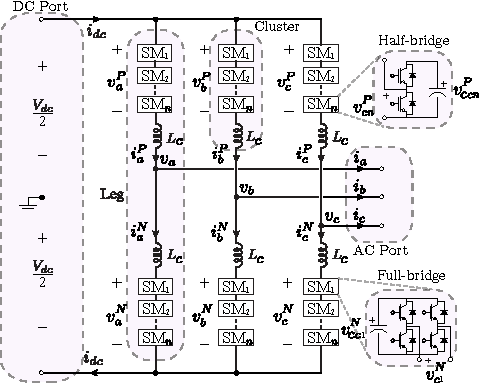
\includegraphics[width=0.7\hsize]{MMC}
  \caption{Ejemplo de imagen vectorial.}
  \label{fig:MMC}
\end{figure}

\subsection{Tablas}

También se pueden utilizar tablas, ¡Crearlas es muy fácil!. Puede usar, por ejemplo, el ``creador de tablas online'' \cite{tablesgenerator}.

% Tabla generada con el plugin Excel2Latex
\begin{table}[H] % Importante el H
	\centering
	\caption{Ejemplo de tablas.}
	\begin{tabular}{ccc}
		\hline
		\textbf{Columna 1} & \textbf{Columna 2} & \textbf{Columna 3} \bigstrut\\
		\hline
		$\omega$ & $\nu$ & $\delta$ \bigstrut[t]\\
		$\Phi$ & $\Theta$ & $\varSigma$ \\
		$\Sigma$ & $\epsilon$ & $\psi$ \\
		\hline
	\end{tabular}
	\label{tab:tabla-1}
\end{table}

\subsection{Pseudocódigo}

El pseudocódigo sirve para describir algoritmos de manera detallada y comprensible, sin preocuparse por la sintaxis de un lenguaje de programación específico. Esto permite que los lectores comprendan el flujo lógico del algoritmo y cómo se implementaría en la práctica, sin necesidad de conocer un lenguaje de programación en particular. Además, el pseudocódigo facilita la comunicación de ideas entre escritor y lectores, ya que se centra en los aspectos conceptuales y algorítmicos en lugar de en detalles específicos de implementación.

\begin{algorithm}
\caption{Representación de pseudocódigo de alto nivel de algún algoritmo.}\label{alg:cap}
    \begin{algorithmic}
        \State Calcular un punto inicial factible $u_{0}$.
        \State Definir $\mathcal{V}_{0} = \emptyset $.
        \State $i \gets 0$.
        \While {\textit{true}}
            \If{$\Delta p_{i} = 0$}
                \If{todos los elementos de $\lambda_{i} \geq 0$}
                    \State{$u^{*} \gets u_{i}$}.
                    \State \textbf{break}.
                \Else
                    \State Remover de $\mathcal{V}_{i}$ la restricción con el mínimo $\lambda_{i}$. 
                    \State $u_{i+1} \gets u_{i}$.
                    \State $\mathcal{V}_{i+1} \gets \mathcal{V}_{i}$.
                \EndIf
            \Else
                \State $u_{i+1} \gets u_{i} + \alpha_{i}\Delta p_{i}$.
                \State Crear $\mathcal{V}_{i+1}$ añadiendo la nueva restricción activa.
            \EndIf
            \State $i \gets i+1$.
        \EndWhile
    \end{algorithmic}
\end{algorithm}

\subsection{Referencias bibliográficas}

\index{referencias}\index{BibTeX}
Todo concepto o idea tomado de otros autores contar con la respectiva
referencia. En redacción técnica de ingeniería rara vez se utiliza la cita
textual, así que es necesario reformular las ideas y conceptos con palabras
propias. En ingeniería electrónica se utilizan los formatos de referencia de la
IEEE o la ACM, que son numéricos, encerrados entre paréntesis cuadrados (por
ejemplo, ``En \cite{Davis1963} se propuso un nuevo algoritmo'', o ``En
\cite{ProakisManolakis1998} los autores proponen tomar las ventajas de los
algorimos presentados en \cite{Oppenheim1998,Roberts2005,Haykin2001} por medio
del método de Newton \cite{Burrus1998} conocido en el área de optimización
lineal.''). La referencia es parte de las frases, así que si la frase termina
con la referencia para indicar la idea, ésta debe estar antes del punto final o
demás signos de puntuación: ``La capacidad de memoria también sigue una Ley
similar a la de Moore \cite{Octave}. Los siguientes son los aspectos a tomar en
cuenta en el diseño del sistema \cite{Lindner2002}:''

Se recomienda utilizar BibTeX para administrar las referencias bibliográficas.


  \include{solucion}
  \include{resultados}
  \include{conclusiones}

  %----------------------------------------------------------------------------
  \bibliographystyle{sty/IEEEtranTIE}
  \bibliography{literatura}

  %----------------------------------------------------------------------------
  \appendix
  \chapter{Apéndices y Anexos}

%% \section{Apéndice A: Preguntas de la entrevista a cliente (Equipo de grupo MACS)}

\begin{enumerate}
    \item Desde sus experiencias con las plataformas USV del laboratorio, ¿cómo describirían su estado actual, y qué aspectos no se pueden modificar o deben preservarse al integrar hardware nuevo?
    \item ¿Qué tareas o misiones les gustaría que estas plataformas pudieran realizar que hoy no pueden?
    \item ¿Qué tipo de datos o resultados esperarían obtener al final de una misión?
    \item ¿Qué tipo de información ambiental les interesaría que el sistema pudiera medir durante una misión?
    \item ¿Dónde y cómo se instalarían físicamente los sensores y el hardware nuevo en el USV, y qué restricciones de peso, tamaño, consumo energético o pruebas de lastre debemos considerar?
    \item ¿Qué tan crítico es que los datos de los sensores estén sincronizados con la posición del vehículo en el momento de la captura?
    \item ¿Han considerado o descartado algún tipo de sensor de percepción hasta ahora? ¿Por qué?
    \item ¿Qué alcance y tipo de comunicación esperan entre los USVs y la estación base, considerando los cuerpos de agua de prueba?
    \item ¿Qué información necesitan recibir en tiempo real en la estación base durante una misión, y qué tan crítico es mantener esa conexión sin interrupciones?
    \item ¿Con qué frecuencia o continuidad necesitarían que se recolecten datos?
    \item Si tuvieran que definir cuándo una misión se considera “exitosa”, ¿qué tendría que pasar?
    \item ¿Qué margen de error en la ubicación o trayectoria, y qué porcentaje de fallas, considerarían aceptables antes de decir que el sistema no es confiable?
    \item ¿Existe algún estándar o referencia que ya usen para evaluar el desempeño de sistemas similares?
    \item ¿Qué condiciones del entorno, requisitos normativos o de seguridad, y permisos deben tenerse en cuenta para operar y probar el sistema, tanto en el laboratorio como en cuerpos de agua reales?
    \item Si un robot fallara o se perdiera durante una misión, ¿qué pasaría después? ¿existe alguna forma de localizarlo o recuperarlo?
    \item ¿Qué limitaciones de tiempo, presupuesto o recursos se deben considerar?
    \item Si tuvieran que elegir entre que el sistema sea más preciso o más fácil de operar, ¿cuál priorizarían, y por qué?
    \item Una vez finalizado este proyecto, ¿cómo se imaginan que el grupo seguiría usando o ampliando el sistema?
\end{enumerate}



  %----------------------------------------------------------------------------
  \backmatter
  \printindex

\end{document}
